%
% This is the LaTeX template file for lecture notes for EE 382C/EE 361C.
%
% To familiarize yourself with this template, the body contains
% some examples of its use.  Look them over.  Then you can
% run LaTeX on this file.  After you have LaTeXed this file then
% you can look over the result either by printing it out with
% dvips or using xdvi.
%
% This template is based on the template for Prof. Sinclair's CS 270.

\documentclass[twoside]{article}
\usepackage{graphics}
\setlength{\oddsidemargin}{0.25 in}
\setlength{\evensidemargin}{-0.25 in}
\setlength{\topmargin}{-0.6 in}
\setlength{\textwidth}{6.5 in}
\setlength{\textheight}{8.5 in}
\setlength{\headsep}{0.75 in}
\setlength{\parindent}{0 in}
\setlength{\parskip}{0.1 in}

%
% The following commands set up the lecnum (lecture number)
% counter and make various numbering schemes work relative
% to the lecture number.
%
\newcounter{lecnum}
\renewcommand{\thepage}{\thelecnum-\arabic{page}}
\renewcommand{\thesection}{\thelecnum.\arabic{section}}
\renewcommand{\theequation}{\thelecnum.\arabic{equation}}
\renewcommand{\thefigure}{\thelecnum.\arabic{figure}}
\renewcommand{\thetable}{\thelecnum.\arabic{table}}

%
% The following macro is used to generate the header.
%
\newcommand{\lecture}[4]{
	\pagestyle{myheadings}
	\thispagestyle{plain}
	\newpage
	\setcounter{lecnum}{#1}
	\setcounter{page}{1}
	\noindent
	\begin{center}
		\framebox{
			\vbox{\vspace{2mm}
				\hbox to 6.28in { {\bf EE 382C/361C: Multicore Computing
						\hfill Fall 2016} }
				\vspace{4mm}
				\hbox to 6.28in { {\Large \hfill Lecture #1: #2  \hfill} }
				\vspace{2mm}
				\hbox to 6.28in { {\it Lecturer: #3 \hfill Scribe: #4} }
				\vspace{2mm}}
		}
	\end{center}
	\markboth{Lecture #1: #2}{Lecture #1: #2}
	%{\bf Disclaimer}: {\it These notes have not been subjected to the
	%usual scrutiny reserved for formal publications.  They may be distributed
	%outside this class only with the permission of the Instructor.}
	\vspace*{4mm}
}

%
% Convention for citations is authors' initials followed by the year.
% For example, to cite a paper by Leighton and Maggs you would type
% \cite{LM89}, and to cite a paper by Strassen you would type \cite{S69}.
% (To avoid bibliography problems, for now we redefine the \cite command.)
% Also commands that create a suitable format for the reference list.
\renewcommand{\cite}[1]{[#1]}
\def\beginrefs{\begin{list}%
		{[\arabic{equation}]}{\usecounter{equation}
			\setlength{\leftmargin}{2.0truecm}\setlength{\labelsep}{0.4truecm}%
			\setlength{\labelwidth}{1.6truecm}}}
	\def\endrefs{\end{list}}
\def\bibentry#1{\item[\hbox{[#1]}]}

%Use this command for a figure; it puts a figure in wherever you want it.
%usage: \fig{NUMBER}{SPACE-IN-INCHES}{CAPTION}
\newcommand{\fig}[3]{
	\vspace{#2}
	\begin{center}
		Figure \thelecnum.#1:~#3
	\end{center}
}
% Use these for theorems, lemmas, proofs, etc.
\newtheorem{theorem}{Theorem}[lecnum]
\newtheorem{lemma}[theorem]{Lemma}
\newtheorem{proposition}[theorem]{Proposition}
\newtheorem{claim}[theorem]{Claim}
\newtheorem{corollary}[theorem]{Corollary}
\newtheorem{definition}[theorem]{Definition}
\newenvironment{proof}{{\bf Proof:}}{\hfill\rule{2mm}{2mm}}

% **** IF YOU WANT TO DEFINE ADDITIONAL MACROS FOR YOURSELF, PUT THEM HERE:
\usepackage{listings}
\usepackage{graphicx}
\begin{document}
	%FILL IN THE RIGHT INFO.
	%\lecture{**LECTURE-NUMBER**}{**DATE**}{**LECTURER**}{**SCRIBE**}
	\lecture{21}{November 8}{Vijay Garg}{Shengwei Wang}
	%\footnotetext{These notes are partially based on those of Nigel Mansell.}
	
	% **** YOUR NOTES GO HERE:
	
	% Some general latex examples and examples making use of the
	% macros follow.  
	%**** IN GENERAL, BE BRIEF. LONG SCRIBE NOTES, NO MATTER HOW WELL WRITTEN,
	%**** ARE NEVER READ BY ANYBODY.
	\section{Transaction Memory}

	\subsection{Transaction}
	For transcations:
	\begin{itemize}
		\item Atomicity
		\item Consistency
		\item Isolation
		\item Durability
	\end{itemize}
	For TM, we are looking at ACI.

	Generally, a transaction can be described as:
	\begin{center}
		\begin{lstlisting}[language=Java]
		begin transaction
			read(x);
			write(z);
			read(y);
			...
		end transaction
		\end{lstlisting}
	\end{center}

	There are several read/write operations.
	
	\subsection{Serializability}

	The execution is equivalent to some series execution of all transactions.

	Databases use locks, but not necessary for programmers.

	\begin{center}
		\begin{lstlisting}[language=Java]
		atomic {
			x = 2;
			while()
			...
		}
		\end{lstlisting}
	\end{center}

	Former structure : 
	\begin{center}
		\begin{lstlisting}[language=Java]
		synchronized (this) {
				...
			}
		\end{lstlisting}
	\end{center}
	
	Difference : By using synchronized key word, we are actually acquiring locks. 

	\begin{center}
		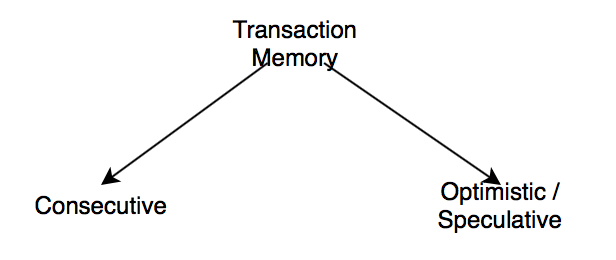
\includegraphics[scale=0.7]{tm.png}
	\end{center}

	When we use locks, we may have problems:
	\begin{itemize}
		\item Deadlocks
		\item Composability Problem
	\end{itemize}

	Example for Composability Problem : 
	
	BLOCKING QUEUE q1, q2


	To do : get item from either of the queue if not empty. 


	Problem : when we do q1.deq(), and q1 is empty, then blocking.

	\subsection{Opacity}
	An execution satisfies opacity if all the committed transactions and the read prefix of the aborted transactions appear as if they have been executed serially in agreement with real-time occurrence order.

	\begin{center}
		\begin{lstlisting}[language=Java]
		Var x, y init 0

		atomic {
			x++;
			y++;
		}

		atomic {   //Zombie Transaction
			if (x != y) {
				while (true);
			}
		}
		\end{lstlisting}
	\end{center}
	

	
	\section{Software Transaction Memory}
	There are multiple algorithms.\\
	Deuce STM (Software Transaction Memory)
	
	In hardware TM:
	\begin{center}
		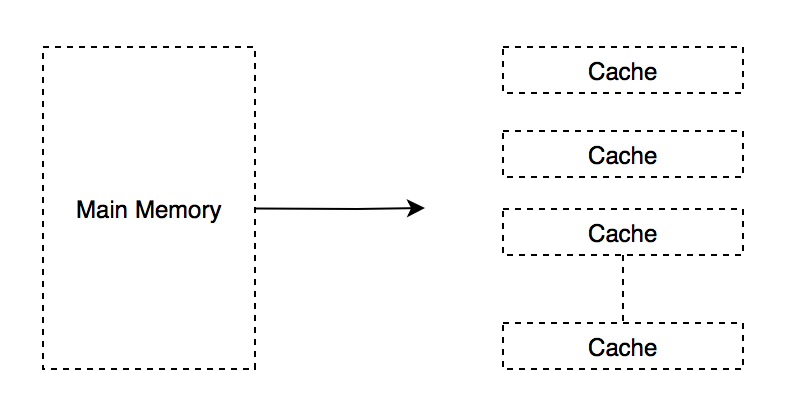
\includegraphics[scale=0.7]{cache.png}
	\end{center}
	we store data from memory to cache. When abort, we just throw away data in cache.
	
	TL2
	\subsection {Key Notion}

	\begin{itemize}
		\item fetch\&add
		\item Clock
		\item Local copies
		\item Dates of local copies
	\end{itemize}

	Put timestamp for each transaction. If the birthday of transaction 1 if 75, and the birthday of transaction 2 is 80, then transaction 1 is completely earlier than transaction 2.

	\begin{itemize}
		\item read set of transaction : lrst
		\item write set of transaction : lwst
		\item local copy : lc (xx)
	\end{itemize}
	
	
	

	\subsection {operations}

	Begin of transcaion
	\begin{center}
		\begin{lstlisting}[language=Java]
		begint()
		lrst <- {}; lwst <- {};
		birthday(T) = clock + 1; //atomic
		\end{lstlisting}
	\end{center}

	Read opreation: X.read()
	\begin{center}
		\begin{lstlisting}[language=Java]
		if there is a local copy of xx
		then 
			return lc(xx).value
		else
			lc(xx) <- copy of xx from shared memory
			if lc(xx).date < birthday(T)
			then 
				lrst(T) <- lrst(T) U {x};
				return lc(xx).value
			else
				abort
		\end{lstlisting}
	\end{center}

	Write operation: X.write(v)
	\begin{center}
		\begin{lstlisting}[language=Java]
		if there is no local copy then allocate space for lc(xx)
		loc(xx).value <- v;
		lwst <- lwst U {x}
		\end{lstlisting}
	\end{center}

	Commit operation : Commit()
	\begin{center}
		\begin{lstlisting}[language=Java]
		lock all x in lrst, lwst
		for all xx <- lrst do
			if xx.date >= birthdate (T)
			then 
				release lock;
				abort
		write_date <- clock.fetch&add();
		for all xx <- lwst do
			xx <- (lc(xx), write_date);

		unlock;
		return commit;
		\end{lstlisting}
	\end{center}

	The algorithm is slow because of making local copies
	When abort, start over again.

	\section{Stream Programming}

	It's like functional programming.\\
	Parallelism is easy if objects don't change.
	\begin{itemize}
		\item lamda function : nameless function
		\item streams
		\item parallel stream
	\end{itemize}

	lamda Funtion :

	\begin{center}
		\begin{lstlisting}[language=Java]
		//using lamda function as the second parameter
		Arrays.sort(data, (a,b) -> (b - a)); 
		\end{lstlisting}
	\end{center}

	Stream : Think in high level
	\begin{center}
		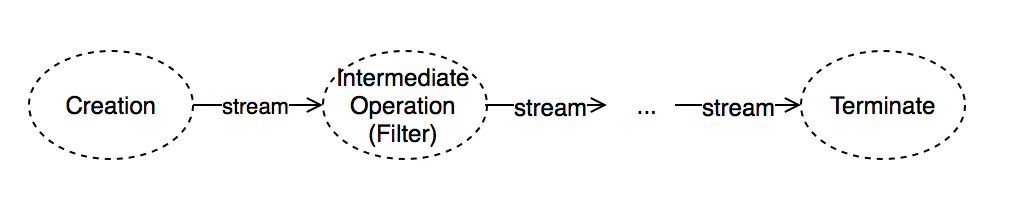
\includegraphics[scale=0.7]{stream.png}
	\end{center}


	
\end{document}